\documentclass[border=5mm]{standalone}
\usepackage{tikz}
\usetikzlibrary{arrows.meta, calc, positioning, decorations.pathreplacing}
\usepackage{amsmath, amssymb}
\renewcommand{\familydefault}{\sfdefault}

% palette distinct from trust-science figure (Okabe-Ito)
\definecolor{policyobs}{HTML}{355070}   % slate blue
\definecolor{policydown}{HTML}{C1663C}  % terracotta
\definecolor{policyup}{HTML}{2A9D8F}    % teal
\definecolor{panelbg}{HTML}{F4F6F8}     % light grey

\begin{document}
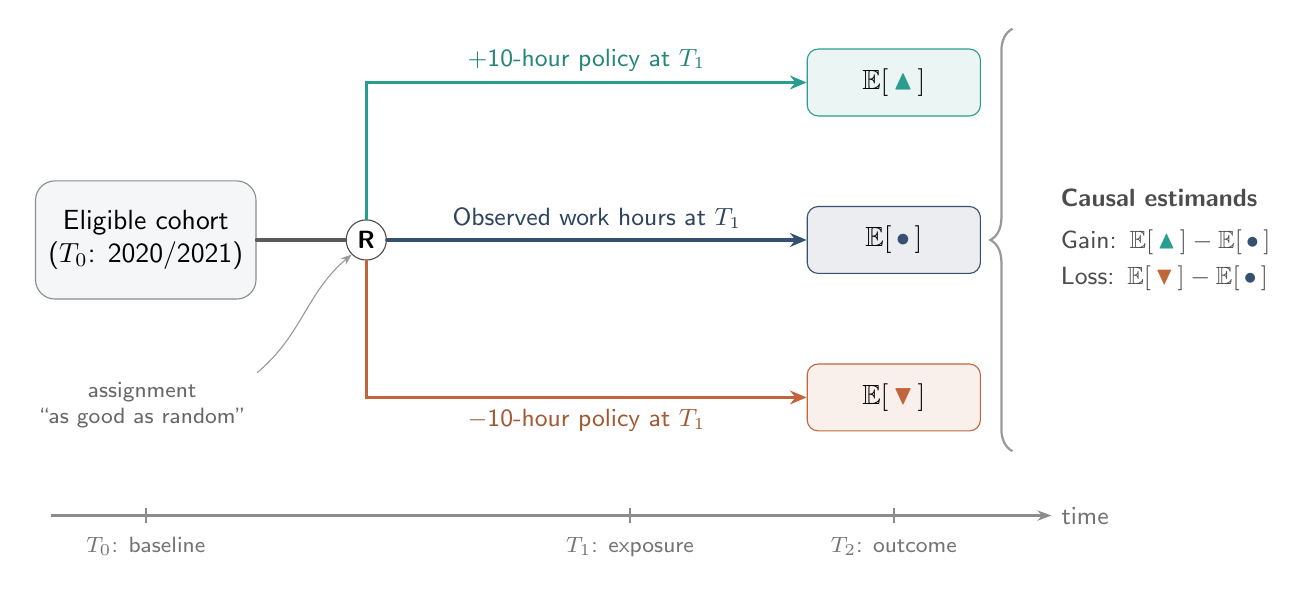
\begin{tikzpicture}[
  every node/.style={font=\normalsize, text=black},
  flow/.style={-{Stealth[length=6pt, width=5pt]}, very thick, line cap=round},
  guide/.style={-{Stealth[length=4pt, width=3pt]}, thin, black!40},
  labelsmall/.style={font=\footnotesize\sffamily, black!60, align=center},
  outcome/.style={
    rounded corners=4pt, minimum width=2.2cm, minimum height=0.85cm,
    align=center, font=\normalsize
  },
  pathlabel/.style={font=\small\sffamily, inner sep=2pt}
]

% baseline cohort
\node[draw=black!45, rounded corners=7pt, fill=panelbg,
  minimum width=2.8cm, minimum height=1.5cm,
  align=center, font=\normalsize\sffamily] (base) at (0,0)
  {Eligible cohort\\($T_0$: 2020/2021)};

% randomisation fork
\node[circle, draw=black!70, fill=white, inner sep=2pt,
  font=\small\bfseries\sffamily] (R) at (2.8,0) {R};

% stem
\draw[very thick, black!65, line cap=round] (base.east) -- (R);

% outcome nodes (spread vertically)
\node[outcome, draw=policyup, fill=policyup!10] (yup) at (9.5, 2.0)
  {$\mathbb{E}[\,\textcolor{policyup}{\blacktriangle}\,]$};
\node[outcome, draw=policyobs, fill=policyobs!10] (yobs) at (9.5, 0)
  {$\mathbb{E}[\,\textcolor{policyobs}{\bullet}\,]$};
\node[outcome, draw=policydown, fill=policydown!10] (ydown) at (9.5, -2.0)
  {$\mathbb{E}[\,\textcolor{policydown}{\blacktriangledown}\,]$};

% elbow knee coordinates
\coordinate (gain-knee) at (R |- yup);
\coordinate (loss-knee) at (R |- ydown);

% elbow paths (up/down then horizontal)
\draw[flow, policyup] (R.north) -- (gain-knee) -- (yup.west);
\draw[flow, policyobs] (R.east) -- (yobs.west);
\draw[flow, policydown] (R.south) -- (loss-knee) -- (ydown.west);

% path labels (centred on horizontal segments)
\node[pathlabel, text=policyup!85!black, anchor=south, yshift=2pt]
  at ($(gain-knee)!0.5!(yup.west)$) {$+$10-hour policy at $T_1$};
\node[pathlabel, text=policyobs!85!black, anchor=south, yshift=2pt]
  at ($(R.east)!0.5!(yobs.west)$) {Observed work hours at $T_1$};
\node[pathlabel, text=policydown!85!black, anchor=north, yshift=-2pt]
  at ($(loss-knee)!0.5!(ydown.west)$) {$-$10-hour policy at $T_1$};

% assignment annotation
\node[labelsmall, below left=1.5cm and 1.2cm of R] (Rlabel)
  {assignment\\``as good as random''};
\draw[guide] (Rlabel.north east) to[out=40, in=220] (R.south west);

% estimand brace (right of outcomes — curly brace, not double-headed arrows)
\draw[decorate, decoration={brace, amplitude=8pt, mirror}, thick, black!40]
  ([xshift=0.4cm, yshift=0.25cm] yup.north east) --
  ([xshift=0.4cm, yshift=-0.25cm] ydown.south east)
  coordinate[midway, right=14pt] (bracemid);

\node[font=\small\sffamily, black!70, align=left, anchor=west] at (bracemid) {%
  \textbf{Causal estimands}\\[4pt]
  Gain:\enspace $\mathbb{E}[\,\textcolor{policyup}{\blacktriangle}\,] - \mathbb{E}[\,\textcolor{policyobs}{\bullet}\,]$\\[2pt]
  Loss:\enspace $\mathbb{E}[\,\textcolor{policydown}{\blacktriangledown}\,] - \mathbb{E}[\,\textcolor{policyobs}{\bullet}\,]$
};

% time axis
\draw[-{Stealth[length=5pt]}, thick, black!45]
  ([xshift=-1.2cm] base |- 0,-3.5) -- ([xshift=2cm] yobs |- 0,-3.5)
  node[right, font=\small\sffamily, black!55] {time};

\draw[thick, black!45] (base |- 0,-3.4) -- (base |- 0,-3.6);
\node[font=\footnotesize\sffamily, black!55, anchor=north]
  at (base |- 0,-3.65) {$T_0$: baseline};

\coordinate (midpath) at ($(R)!0.5!(yobs)$);
\draw[thick, black!45] (midpath |- 0,-3.4) -- (midpath |- 0,-3.6);
\node[font=\footnotesize\sffamily, black!55, anchor=north]
  at (midpath |- 0,-3.65) {$T_1$: exposure};

\draw[thick, black!45] (yobs |- 0,-3.4) -- (yobs |- 0,-3.6);
\node[font=\footnotesize\sffamily, black!55, anchor=north]
  at (yobs |- 0,-3.65) {$T_2$: outcome};

\end{tikzpicture}
\end{document}
